\section{Theory}

\begin{frame}
  \frametitle{Summary}
  \tableofcontents[currentsection]
\end{frame}

\subsection{Presentation}

\begin{frame}{Motivations}
  \begin{block}{Algorithmic problems}
    \begin{itemize}
      \item Stochastic
      \item Convergence
    \end{itemize}
  \end{block}

  \begin{block}{Modelization problems}
    \begin{itemize}
      \item How to encode a problem?
      \item Size of the initial population?
      \item Mutation operator?
      \item Recombination operator?
      \item Individual selection?
    \end{itemize}
  \end{block}
\end{frame}

\subsection{Schemata Theorem}
\begin{frame}{Schemata}
  \begin{block}{Goal}
    \begin{itemize}
    \item Defined by J.Holland in 1975\cite{holland1992}.
    \item Represent a group of individual who all share some characteristics.
    \item One schema, two schemata ;)
    \end{itemize}
  \end{block}

  \begin{block}{Definition}
    \begin{itemize}
    \item Defined on the alphabet: $\{0;1;\#\}$
    \item $\#$ is "Don't care": it can be 0 or 1
    \end{itemize}
  \end{block}
\end{frame}

\begin{frame}{Example and measures}
  \begin{block}{Example}
    \begin{itemize}
    \item The schema: $H = 1\textcolor{red}{\#}10\textcolor{red}{\#}1\textcolor{red}{\#}$
    \item Represents the following individuals:
      \begin{center}
        $1\textcolor{red}{0}10\textcolor{red}{0}1\textcolor{red}{0}$,
        $1\textcolor{red}{0}10\textcolor{red}{0}1\textcolor{red}{1}$,
        $1\textcolor{red}{0}10\textcolor{red}{1}1\textcolor{red}{0}$,
        $1\textcolor{red}{0}10\textcolor{red}{1}1\textcolor{red}{1}$,
        $1\textcolor{red}{1}10\textcolor{red}{0}1\textcolor{red}{0}$,
        $\ldots$
      \end{center}
    \end{itemize}
  \end{block}

  \begin{block}{Measures}
    \begin{itemize}
      \item Order(o): number of fixed positions
      \item Defining length($\delta$): distance between the first and last defined positions.
      \item Here: $o(H) = 4$ and $\delta(H) = 5$
      \item Intuitively: schemata with low o and short $\delta$ have an higher probability of surviving from a generation to the next.
    \end{itemize}
  \end{block}
\end{frame}

\begin{frame}{Graphical representation}
  \begin{center}
    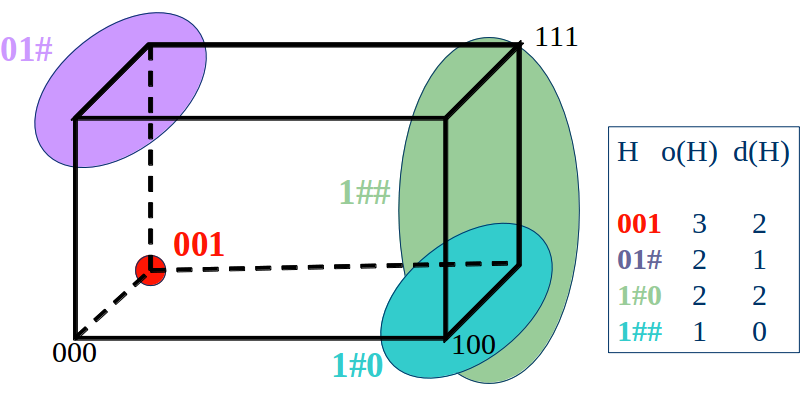
\includegraphics[scale=.4]{img/schema}
  \end{center}
\end{frame}

\begin{frame}{Possible evolutions : selection}
  \begin{block}{Hypothesis}
    \begin{itemize}
    \item Assume a fitness proportional reproduction
    \item $$\mathds{P}(x,t+1) = \frac{f(x)}{\bar{f(t)}}$$
    \end{itemize}
  \end{block}

  \begin{block}{Transmission of a schema}
    $$\begin{array}{lll}
      E(m(H,t+1)) & = & \sum\limits_{x \in H} \frac{f(x)}{\bar{f(t)}}\\
      & = & m(H,t) \times \frac{f(H,t)}{\bar{f(t)}}\\
    \end{array}$$
  \end{block}
\end{frame}

\begin{frame}{Disruptions}
  \begin{block}{Mutation}
    \begin{itemize}
    \item bit-wise mutations with probability $p_m$
    \item Mutation events are independant
    \item $\mathds{P}_{Smuta}(H) \geq (1 - p_m)^{o(H)}$
    \end{itemize}
  \end{block}

  \begin{block}{Crossover}
    \begin{itemize}
      \item One point crossover with probability $p_c$
      \item l - 1 possible crossover points
      \item $\mathds{P}_{Scross}(H) \geq (1 - p_c \times \frac{\delta(H)}{l - 1})$
    \end{itemize}
  \end{block}
\end{frame}

\begin{frame}{Schema theorem}
  \begin{block}{Theorem}
    $$E(m(H,t+1)) \geq \underbrace{m(H,t) \times \frac{f(H,t)}{\bar{f(t)}}}_{\mathds{P}(x,t+1)}
    \underbrace{\times (1 - p_c \times \frac{\delta(H)}{l-1})\vphantom{\frac{f(H,t)}{\bar{f(t)}}}}_{\mathds{P}_{Smuta}}
    \underbrace{\times (1 - p_m)^{o(H)}\vphantom{\frac{f(H,t)}{\bar{f(t)}}}}_{\mathds{P}_{Scross}}$$
  \end{block}

  \begin{block}{Limitations}
    \begin{itemize}
      \item Only a lower bound
      \item Expectation
      \item Works with infinite population
      \item Convergence?
      \item Very strong hypothesis
    \end{itemize}
  \end{block}
\end{frame}

\begin{frame}{Building Block hypothesis}
  \begin{block}{Presentation}
    \begin{itemize}
    \item Tightly linked to schema theorem
    \item Try to explain why does EA works
    \end{itemize}
  \end{block}

  \begin{block}{BBH}
    "A genetic algorithm seek near optimal performance through the juxtaposition of short, low-order, high-performance schemata"\cite{goldberg1989}
  \end{block}

  \begin{block}{But...}
    \begin{itemize}
      \item Skepticism
      \item Theoretically\cite{wright2003}
      \item Experimentally\cite{forrest1993}
    \end{itemize}
  \end{block}
\end{frame}

\section{Schemata extension}
\begin{frame}{Extension to GP}
  \begin{block}{Goal}
    Give a meaningful schema definition for tree representation.
  \end{block}

  \begin{block}{Problems}
    \begin{itemize}
      \item Not a linear structure
      \item Larger alphabet
      \item How to interpret \# (don't care)?
      \item How to keep correct o and $\delta$ measures?
    \end{itemize}
  \end{block}
\end{frame}

\begin{frame}{Koza's schema}
  \begin{block}{Schema definition}
    \begin{itemize}
      \item Non-positional list of S-expressions that can be match anywere in the tree.\cite{Koza92}
      \item Example: H = [(- 2 x), x] matches all the programs that have at least one of each expressions.
    \end{itemize}
  \end{block}

  \begin{center}
    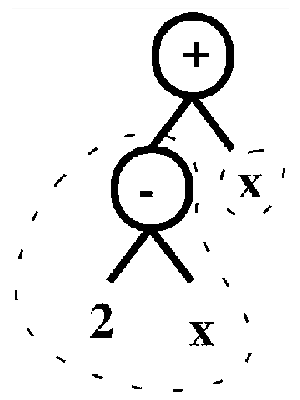
\includegraphics[scale=0.90]{img/schemak}\\
    The program (+ (- 2 x) x)
  \end{center}

  \begin{block}{Pro/Cons}
    \begin{itemize}
      \item<pro@1> An equation has been given for the schema theorem on those schema
      \item<con@1> No order nor defining length
    \end{itemize}
  \end{block}

\end{frame}

\begin{frame}{O'Reilly's schema}
  \begin{block}{Schema definition}
    \begin{itemize}
      \item Multi-set of subtrees and tree fragments (i.e. a subtree with a \# node)\cite{oreilly1994}
      \item Example: H = [(+ \# x), x, x] matches any tree with at least one subtree of the form (+ \# x) and two subtrees equals to $x$
    \end{itemize}
  \end{block}

  \begin{center}
    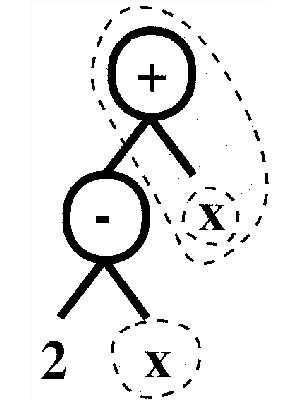
\includegraphics[scale=0.90]{img/schemar}\\
    The program (+ (- 2 x) x)
  \end{center}

    \begin{block}{Pro/Cons}
      \begin{itemize}
        \item<pro@1> $o(H)$ : number of nodes corresponding to s-expression and fragments
        \item<con@1> no schema theorem nor $\delta$
      \end{itemize}
    \end{block}
\end{frame}

\subsection{More theory}
\begin{frame}{Gettin' higher}
  \begin{block}{Canonical GA}
    \begin{itemize}
    \item Holland 1975
    \item Discrete non-overlapping generations
    \item frequency independant selection
    \item infinite population size
    \item Three steps: selection, random mating, reproduction
    \end{itemize}
  \end{block}

  \begin{block}{Dynamical equation}
    $$p(x,t+1) = \sum\limits_{x,y \in S} T(x \leftarrow y,z)
    \frac{f(y)f(z)}{\bar{f(t)}^2}p(y,t)p(z, t)$$

    where :
    \begin{itemize}
      \item p(x,t) is the proportion of string x at time t
      \item S is the search space
      \item $T(x \leftarrow y,z)$ is the transmission function, the probability of getting x with parents y and z.
    \end{itemize}
  \end{block}
\end{frame}

\begin{frame}{Measurement function}
  \begin{block}{Goal}
    Extract the macroscopic dynamic of the population for its microscopic (dynamical equation).
  \end{block}

  \begin{block}{Definition}
    \begin{itemize}
    \item$M: S \times P \longrightarrow \nu$
      \begin{itemize}
        \item S is the search space
        \item P is a parameter family
        \item $\nu$ is a vector space (typically $\mathbb{R}^k$)
      \end{itemize}
    \item Example: f, the fitness function is a measurement function
    \end{itemize}
  \end{block}

  \begin{block}{Changes in average}
    \begin{itemize}
    \item Change in the population average of a measurement function is a measure of how the population is evolving
    \item $\bar{M_t} = \sum\limits_{x} M_t(x)p(x,t)$
    \item $\bar{M_{t+1}} = \sum\limits_{x} M_t(x)p(x,t+1)$
    \end{itemize}
  \end{block}
\end{frame}

\begin{frame}{Price's theorem}
  \begin{block}{Covariance and Selection}
    \begin{center}
      $\forall y,z \; \phi(y,z) = \sum\limits_{x} M(x)T(x \leftarrow y,z)$\\ expected value of M among (y,z)'s offspring
      \end{center}
  \end{block}

  \begin{block}{Next generation}
    $$\bar{M_{t+1}} = \bar{\phi}
    + Cov[\phi(y,z), \frac{f(y)f(z)}{\bar{f}^2}]$$
    where:
    \begin{itemize}
    \item $\bar{\phi} = \sum\limits_{y,z} \phi(y,z)p(y)p(z)$ avg. offspring value without selection
    \item $Cov[\phi(y,z), \frac{f(y)f(z)}{\bar{f}^2}] =
      \sum\limits_{y,z} \phi(y,z) \frac{f(y)f(z)}{\bar{f}^2}p(y)p(z) -
      \bar{\phi}$ population covariance over the distribution of genotype
    \end{itemize}
  \end{block}

  \begin{block}{Interpretation}
    Covariance between parental and offspring fitness is the means by which selection directs the evolution of the population
  \end{block}
\end{frame}

\begin{frame}{Schema theorem is back}
  \begin{block}{Thanks to Price's theorem}
    \begin{itemize}
      \item if $M(x, H) = \left\{\begin{array}{l}
        1 \text{ if } x \in H\\
        0 \text{ otherwise}
        \end{array}
        \right .$
      \item and $\phi(y,z,H) = \sum\limits_{x} M(x,H)T(x \leftarrow y,z)$
      \item then $p(H) = \bar{M(H)}$
    \end{itemize}
  \end{block}

  \begin{block}{Schema frequency change\cite{Altenberg95}}
    $$p(H,t+1) = \bar{\phi(H)} + Cov[\phi(y,z,H), \frac{f(y)f(z)}{\bar{f}^2}]$$
  \end{block}

\end{frame}

\begin{frame}{Conclusion}

  \begin{block}{On genetic algorithm}
    \begin{itemize}
    \item GA possess a theoretical basis since the beginning
    \item The Schema theorem is very controversial
    \item But still widely present and used
    \end{itemize}
  \end{block}

  \begin{block}{On schema}
    \begin{itemize}
      \item Correctly defined over a fixed-length binary alphabet: $\{0,1\}^l$
      \item Different schema definitions for tree syntax
      \item More? Whigham's schema for context-free-grammar\cite{whigham1995}
    \end{itemize}
  \end{block}
\end{frame}

\begin{frame}{Going further}
  \begin{block}{Limitations}
    \begin{itemize}
      \item Theory does not give a simple and direct insight about how to model a problem
      \item Other weird effects can appear (ex: Boast)
    \end{itemize}
  \end{block}

  \begin{block}{Other theoretical tools}
    \begin{itemize}
      \item Markov chains
      \item Landscape analysis
    \end{itemize}
  \end{block}
\end{frame}
